\chapter{Introduction to Operational Amplifiers}
One of the major functions of circuits is to amplify signals. This means that the output amplitude is made greater than the input amplitude. To borrow the language of the last chapter, amplification would make the frequency response of such a system greater than 1, which we saw could not happen with passive circuits involving just capacitors, inductors, and resistors. In this chapter, we will introduce a ubiquitous electronic device called the \textbf{operational amplifier} (or \textbf{op amp} for short), which is capable of amplification, filtering, and more. Most circuits today have at least one op amp, and after you read this chapter you will be able to determine what they do in the context of a larger circuit.
\section{Ideal Op Amps}
Figure \ref{firstOpAmp} shows the schematic representation of an op amp by itself. This triangle-shaped symbol obscures the guts of the device, merely showing us its most important externally-accessible nodes. There are so many different implementations of op amps available from electronic suppliers that you might think they all have vastly different characteristics. However, all op amps increase or otherwise change the amplitude of an input voltage signal and they all ideally adhere to the same rules.
\begin{figure}[h!]
\centering
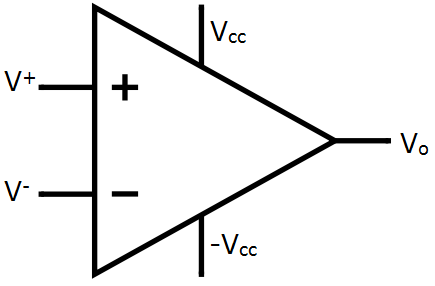
\includegraphics[width=6cm]{figures/loneOpAmp.png}
\caption{The schematic representation of an op amp.}
\label{firstOpAmp}
\end{figure}
\par
Back to the Figure \ref{firstOpAmp}: The two ports on the left are labeled with a ``+'' and a ``-''. These are referred to as the ``non-inverting'' and ``inverting'' inputs, respectively. The input voltage for our amplifier is connected to these inputs, as we will see in the next section. The port at the right of the op amp is where the output for the amplifier comes from. The two ports at the top and bottom of the amplifier are where the power supply for the op amp is connected. Most op amps require two voltage supplies---one that provides a positive voltage and another that provides a negative voltage of equal amplitude.
\par
Now that we know what all those connections are for, let's look at the simplest behavior of this device. When a voltage difference is presented across the input terminals (in other words, if $(V_+-V_-)\neq0$ in Figure \ref{firstOpAmp}), the output voltage is linearly proportional to that input:
$$
V_o = A_{ol}\cdot (V_+-V_-)
$$
In this expression, $A_{ol}$ is the \textbf{open-loop gain} for the op amp, and typical values for $A_{ol}$ are $\sim10^5$. This is extremely large! If the power supply for the op amp allowed it, in this configuration even a very modest input voltage amplitude of 1mV would produce an output voltage amplitude of 100V! In practice, the amplitude of a signal in this configuration is limited by the positive and negative voltage supplies for the op amp (V$_{\textnormal{cc}}$ and -V$_{\textnormal{cc}}$ in Figure \ref{firstOpAmp}); the output voltage of an op amp cannot exceed the positive or negative supply voltages, and if its amplitude would ever exceed those limits, it will be ``clipped'' at the op amp power supply voltages. However, the open-loop gain is an internal property of an op amp that is based on its fabrication parameters and which we cannot change. So, in this configuration, an op amp isn't really very useful. We need a way to ``reign in'' the gain of this device.
\par
Op amps are really useful when we connect their output voltage back to their inverting input in some way. This is called \textbf{negative feedback}, and it is called this because we feed the output back to the negative input. Makes sense, right? When op amps are configured with negative feedback, they obey two rules that we will use to analyze their behavior:
\begin{enumerate}
\item No current flows into or out of the inverting or non-inverting input
\item There is no voltage difference between the input terminals (you can treat the inverting and non-inverting inputs as the same node)
\end{enumerate}
In the next several sections, we will analyze some common configurations of resistive amplifier circuits using the two rules above.
\section{Unity Gain Buffer}
The simplest op amp configuration with negative feedback is known as a \textbf{unity gain buffer}, and its schematic is shown in Figure \ref{unityGainBuffer}.
\begin{figure}[h!]
\centering
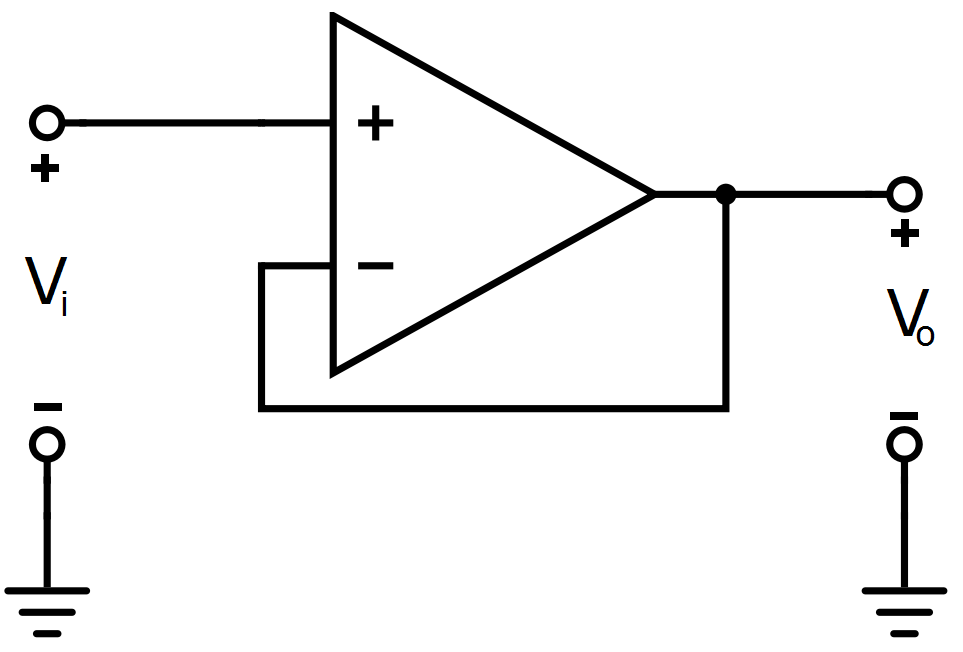
\includegraphics[width=7cm]{figures/unityGainBuffer.png}
\caption{An op amp in the unity gain buffer configuration.}
\label{unityGainBuffer}
\end{figure}
Using the rule that there is no voltage difference between the input terminals of the op amp, we can easily determine that $V_o=V_i$. Why would anyone use one of these? Well, even though we didn't change the input \textit{voltage}, the op amp can ideally drive any load without being affected by that load. Remember when we talked about voltage dividers being loaded down? If we connect a unity gain buffer to the output of a voltage divider, the op amp can then ideally drive any load without that load affecting the voltage. We will revisit this configuration in the next chapter.

\section{Inverting Amplifier}
\begin{figure}[h!]
\centering
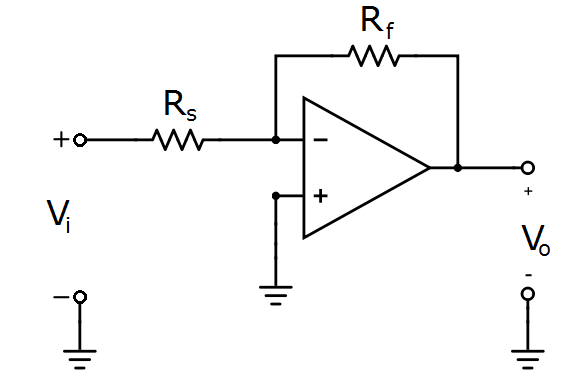
\includegraphics[width=7cm]{figures/invertingAmplifier.png}
\caption{An inverting amplifier op amp configuration.}
\label{invertingAmplifier}
\end{figure}
Let's look at the circuit of Figure \ref{invertingAmplifier}. Note that in this circuit, we have omitted the voltage supply inputs for the op amp. This is common practice when analyzing op amp configurations because it removes unnecessary clutter from the diagram. This circuit incorporates negative feedback through a resistor, $R_f$. Because this circuit has negative feedback, we can use two ideal op amp rules from the last section to determine an expression for the output voltage.
\par
Let's use the second rule of our two op amp rules to declare the inverting input node to be grounded. We can do this because the non-inverting input is grounded, and the second rule states that there is no voltage difference between the two inputs. Therefore, the circuit can be reduced to that shown in Figure \ref{invertingAmplifier2}, where the inverting input is now grounded. 
\begin{figure}[h!]
\centering
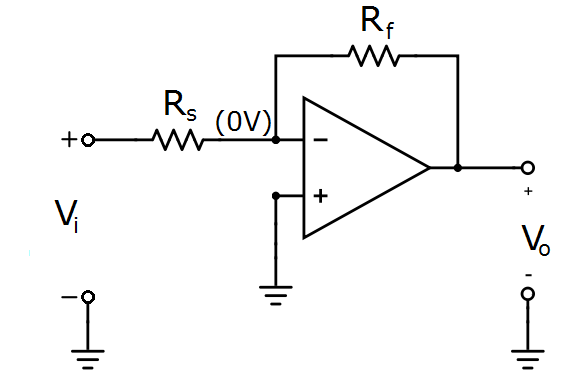
\includegraphics[width=7cm]{figures/invertingAmplifier2.png}
\caption{An inverting amplifier op amp configuration, with both the inputs explicitly grounded.}
\label{invertingAmplifier2}
\end{figure}
\par
Next, taking into account the fact that there is no current flowing into the inverting input allows us to completely remove the op amp as shown in Figure \ref{invertingAmplifier3}. Now we just have to solve for $V_o$ in terms of $V_i$ using the techniques we learned all the way back in Chapter \ref{chap:resistorRulesAndTricks}, because all that remains of our original circuit is a resistor network. I have also labeled this figure with currents $i_s$ and $i_f$ which will be helpful in our analysis.
\begin{figure}[h!]
\centering
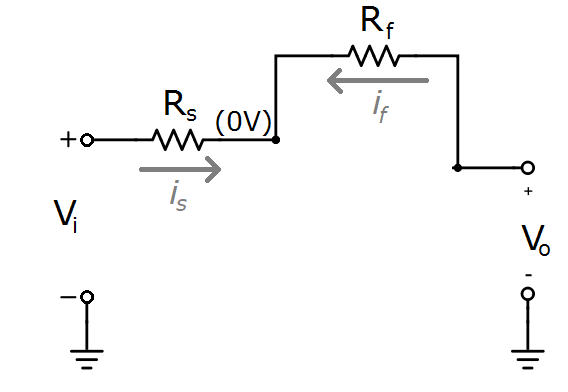
\includegraphics[width=7cm]{figures/invertingAmplifier3.png}
\caption{An inverting amplifier op amp configuration with the op amp removed!}
\label{invertingAmplifier3}
\end{figure}
\par
Let's start by determining how those currents are defined. We can see that according to KVL, the voltage across $R_s$ is $V_i$. Also, according to Ohm's law, $V_i = i_s\cdot R_s$, so $i_s = V_i/R_s$. Next, let's find a definition for $i_f$; by the same logic as before, $V_o = i_f\cdot R_f$, therefore $i_f = V_o/R_f$.
\par
Knowing the definitions for these currents is fine, but we don't want them in our final expression for $V_o$. Notice that at the node between the two resistors in Figure \ref{invertingAmplifier3}, there is a current coming in from the left and a current coming in from the right, but there doesn't appear to be a current flowing out of the node. According to KCL, the current flowing in should be equal to the current flowing out, but if there is no current flowing out, 
$$
i_s + i_f = 0
$$
This means that one of these currents must be negative. That may not seem possible, but a negative current is just a current whose arrow is pointed in the opposite direction from how it actually flows. Let's plug our expressions for these currents into this expression, and then finally solve for $V_o$:
$$
\frac{V_i}{R_s} + \frac{V_o}{R_f} = 0
$$
$$
\frac{V_o}{R_f} = -\frac{V_i}{R_s}
$$
$$
V_o = -\frac{R_f}{R_s}V_i
$$
\par
This expression shows us that the output voltage is a negated version of the input voltage. This amplifier configuration is known as an \textbf{inverting amplifier}, because the output voltage is \textit{inverted} (i.e., negative) with respect to the input voltage. Additionally, the output is scaled by a factor of $R_f/R_s$; these resistors can be chosen so that the scaling factor can have any value we want.
\par
All amplifier systems can be characterized by their \textbf{gain}, and for op amps, we most often refer to \textbf{voltage gain}, which is defined as 
$$
A_V = \frac{V_o}{V_i}
$$
Sometimes $A_V$ is a function of frequency, but for the amplifier of Figure \ref{invertingAmplifier}, the voltage gain is defined as
$$
A_V = -\left(\frac{R_f}{R_s}\right)
$$
Inverting amplifiers are characterized by their negative gain, and you can recognize them schematically by the fact that their input voltage is connected to their inverting input.
\section{Non-Inverting Amplifier}
\begin{figure}[h!]
\centering
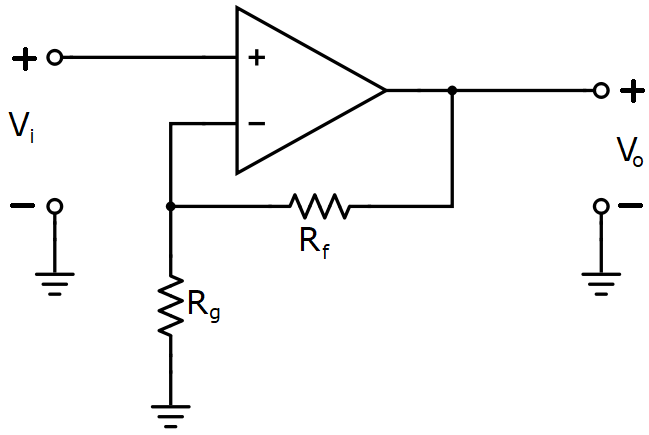
\includegraphics[width=7cm]{figures/nonInvertingAmp.png}
\caption{A non-inverting amplifier circuit.}
\label{nonInvertingAmp}
\end{figure}
Now let's look at the circuit of Figure \ref{nonInvertingAmp}. This circuit has negative feedback, so we can again use the two ideal op amp rules to determine the voltage gain for this amplifier configuration.
\par
The voltage with respect to ground at the non-inverting input to the op amp is $V_i$. Because there is no voltage difference between the inverting and non-inverting inputs for the op amp, we can treat the inverting input voltage as $V_i$, too. Furthermore, given the fact that there is no current flowing into the inputs of the op amp, we can re-draw the circuit without the op amp as shown in Figure \ref{nonInvertingSansAmp}.
\begin{figure}[h!]
\centering
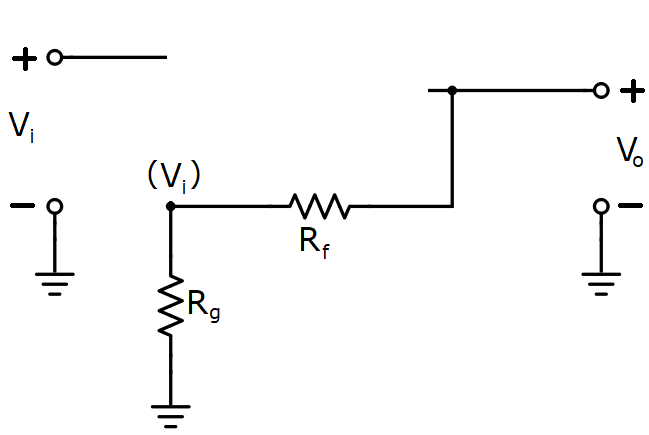
\includegraphics[width=7cm]{figures/nonInvertingSansAmp.png}
\caption{A non-inverting amplifier circuit with the op amp removed.}
\label{nonInvertingSansAmp}
\end{figure}
\par
From this figure, you can see that the resistors make a voltage divider. This voltage divider looks a little strange, however, since $V_i$ is the smaller of the two voltages in this configuration. Nevertheless, we can use the voltage divider rule to relate the input and output voltages:
$$
V_i = V_o\left(\frac{R_g}{R_f+R_g}\right)
$$
Using this expression, we can solve for voltage gain:
$$
A_V = \frac{V_o}{V_i} = \frac{R_f+R_g}{R_g} = 1 + \frac{R_f}{R_g}
$$
This type of amplifier configuration is known as a \textbf{non-inverting amplifier}, because its gain is not inverted. Note that its voltage gain is always at least 1.

\section{Summing Amplifier}
The circuit in Figure \ref{summingAmp} is another common amplifier configuration called a \textbf{non-inverting summing amplifier}. 
\begin{figure}[h!]
\centering
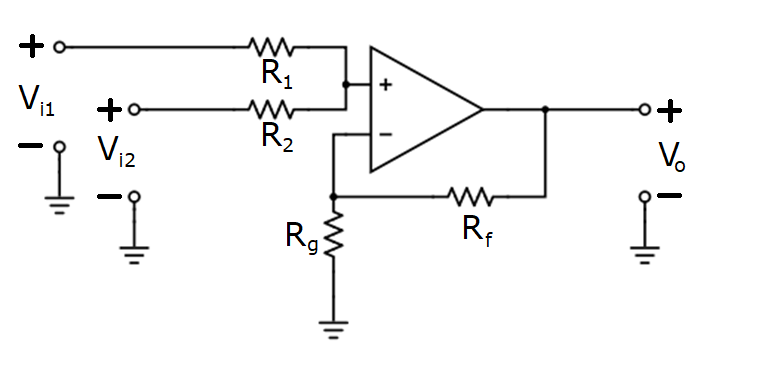
\includegraphics[width=10cm]{figures/nonInvertingSummingAmp.png}
\caption{A summing amplifier circuit.}
\label{summingAmp}
\end{figure}
This circuit has more pieces than the other two configurations we have already looked at, but we can determine its voltage gain in the same way as before. First, we can solve for the inverting input voltage using the voltage divider rule:
$$
V_- = V_o\left(\frac{R_g}{R_g+R_f}\right)
$$
Next, we need to determine the voltage of the non-inverting input. To do so, we will use the fact that only one current can flow between $V_i1$ and $V_i2$, since no current flows into the op amp. Let's call that current $i_{12}$, and let's assume it travels from input $V_i1$ to $V_i2$. We can use this current to deduce a KVL equation for that portion of the circuit, which will ultimately allow us to find an expression for $V_+$:
$$
V_{i1}-i_{12}\cdot R_1 = V_+
$$
We will need one additional equation to eliminate $i_{12}$ from our calculation:
$$
V_{i1}-i_{12}\cdot R_1 - i_{12}\cdot R_2 = V_{i2}
$$
Putting these all together yields
$$
V_- = V_+
$$
$$
V_o\left(\frac{R_g}{R_g+R_f}\right) = V_{i1}-i_{12}\cdot R_1
$$
$$
i_{12} = \frac{V_{i1}-V_{i2}}{R_1 + R_2}
$$
$$
V_o\left(\frac{R_g}{R_g+R_f}\right) = V_{i1}-\frac{V_{i1}-V_{i2}}{R_1 + R_2}\cdot R_1 = \frac{V_{i1}(R_1+R_2)-V_{i1}R_1+V_{i2}R_1}{R_1+R_2}
$$
$$
= \frac{\cancel{V_{i1}R_1}+V_{i1}R_2\cancel{-V_{i1}R_1}+V_{i2}R_1}{R_1+R_2}
$$
And finally, 
$$
V_o = \left(\frac{R_g+R_f}{R_g}\right)\cdot\left( \frac{V_{i1}R_2+V_{i2}R_1}{R_1+R_2}\right)
$$
\par
This is called a summing amplifier for the obvious reason that its output is a weighted sum of the input voltages. There are, of course, several resistors mixed in there, too, but assuming all of the resistors are the same value, 
$$
V_o = \left(\frac{\cancel{2R}}{\cancel{R}}\right)\cdot\left( \frac{V_{i1}\cancel{R}+V_{i2}\cancel{R}}{\cancel{2R}}\right) = V_{i1}+V_{i2}
$$
We could also add more voltages with this same configuration as long as we connect them to the non-inverting input through a resistor. Obviously, it is hard to express the gain of this amplifier configuration in the same way as the previous configurations, since there are multiple input voltages.

\section{Recap: Ideal Op Amp Rules and Resistive Amplifier Configurations}
In this chapter we covered the rules we use for analyzing op amps in circuits. We also looked at a few common configurations for resistive op amp circuits. We will be revisiting some of these in the next chapter, but with capacitors mixed in among the resistive elements. The techniques we used to find the voltage gain and expressions for $V_o$ for the circuits in this chapter apply to the analysis of any op amp circuit. Here is a brief synopsis of the main concepts of this chapter:
\begin{description}
\item[Open-Loop Configuration] This is the case when the output of an op amp is not fed back to the inverting input. The op amp then amplifies any voltage difference between the non-inverting and inverting input terminals to produce its output. The open-loop gain for an op amp is $\sim10^5$, which means even tiny input voltages are amplified to an extreme degree. This configuration has limited uses.
\item[Negative Feedback] happens when the output of an op amp is fed back into its inverting input. This allows us to design circuits with a particular value for the voltage gain as opposed to the open-loop gain.
\item[Ideal Op Amp Rules] are the two rules we assume are true for any op amp in a configuration with negative feedback:
\begin{enumerate}
\item The voltage at the inverting input is the same as the voltage at the non-inverting input
\item No current flows into the inputs of the op amp
\end{enumerate}
With these two rules, we were able to dramatically reduce the complexity of analysis.
\item[Voltage Gain] is defined as 
$$
A_V = \frac{V_o}{V_i}
$$
This is reminiscent of the frequency response of a filter, except that the voltage gain can have a value greater than 1. So far, we have only seen frequency-independent voltage gain, but in the next chapter that will change.
\item[Unity Gain Buffer] This op amp configuration produces an output voltage that is the same as the input voltage; in other words, the voltage gain of this configuration is 1. This configuration is useful for driving loads downstream in the signal path of a circuit.
\item[Inverting Amplifier] This is an amp whose output is negated with respect to its input voltage.
\item[Non-Inverting Amplifier] This is an amplifier whose output is not negated with respect to its input. 
\item[Non-Inverting Summing Amplifier]This configuration takes two or more voltages as inputs and its output is a weighted sum of those inputs. If all the resistors in the circuit are the same, however, the output is just the sum of the inputs.
\end{description}

There are several more resistive configurations for op amps, but in the next chapter we will look at similar circuits to those we saw in this chapter, except with capacitors \textit{and} resistors.